\documentclass{beamer}
\usepackage{graphicx}
\usepackage{tikz}
\usetikzlibrary{shapes,arrows}
\usepackage{tikz}
%\usecolortheme{seahorse}
  \setbeamertemplate{footline}[page number]
\usepackage{multirow}
\setbeamertemplate{navigation symbols}{}
\setbeamertemplate{frametitle}[default][center]
\setbeamerfont{frametitle}{shape=\scshape}
\usepackage{color}

\usepackage{csquotes}

\usepackage{xcolor}

\usepackage[flushleft]{threeparttable}

{\title{\textsc{Econ 352 - Introduction to Macro} \\ \tiny (See Williamson Ch. 1)}
\author{Trevor S. Gallen}
\date{}
\begin{document}
\renewcommand*{\inserttotalframenumber}{\pageref{lastframe}}


\setbeamertemplate{caption}{\raggedright\insertcaption\par}

\begin{frame}
\titlepage
\end{frame}

\begin{frame}
\frametitle[alignment=center]{What is Macro?}
\begin{itemize}
\item Macro is micro with $\Sigma$'s
\bigskip
\item How do collections of microeconomic agents interact?
\bigskip
\begin{itemize}
\item Why are rich countries rich, and poor countries poor (and why does this persist?)
\bigskip
\item Why are we so much richer now than in the past?
\bigskip
\item Why does total production and employment fluctuate so much?
\bigskip
\item Why is there inflation?
\bigskip
\item What causes unemployment?
\end{itemize}
\item It used to be (pre-1970) that Macro was conjecturing equations, estimating them, no microfoundations (nonsense!)
\bigskip
\item Now, (good) modern macro is firmly built up from micro principles
\bigskip
\item Distinction now is in \emph{topic} not models
\end{itemize}
\end{frame}

\begin{frame}
\frametitle[alignment=center]{The rest of this lecture}
\begin{itemize}
\item Give you a \emph{preview} of the things macroeconomists think about, the data that raises many of our questions
\bigskip
\item If a figure doesn't make sense to you, that's okay right now, we'll go in depth later
\end{itemize}
\end{frame}

\begin{frame}
\frametitle[alignment=center]{GDP}
\begin{itemize}
\item GDP is the quantity of goods \& services produced within a country's borders during some specified period of time (\textcolor{red}{a flow!})
\bigskip
\item Because all things produced are also paid for, it's also the quantity of income earned by those contributing to domestic output (preview: ``income approach" vs. ``expenditure")
\bigskip
\item Let's take a look at U.S GDP over time
\end{itemize}
\end{frame}

\begin{frame}
\frametitle[alignment=center]{Real Per Capita GDP over Time}
\begin{figure}
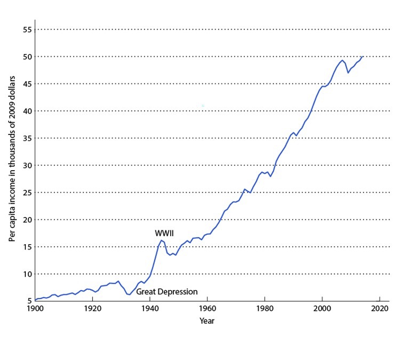
\includegraphics[scale=0.6]{Figures/W_Fig_1pt1.png}
\end{figure}
What do you notice?
\end{frame}

\begin{frame}
\frametitle[alignment=center]{GDP-Things to Notice}
\begin{itemize}
\item Some comments:
\begin{enumerate}
\item Great Depression was big!
\bigskip
\item But growth dwarfs all recessions (an ordinary recession sends us back in time $<$ 2 years)
\bigskip
\end{enumerate}
\item And some questions:  
\begin{enumerate}
\item What causes economic growth?
\item Could economic growth continue indefinitely, or is there some limit?
\item Is there anything that governments can or should do to alter the rate of economic growth?
\item What causes business cycles?
\item Could the dramatic increases and decreases in economic growth that occurred during the Great Depression and World War II be repeated?
\item Should governments act to smooth business cycles?
\end{enumerate}
\end{itemize}
\end{frame}

\begin{frame}
\frametitle[alignment=center]{Thinking more about GDP}
\begin{itemize}
\item GDP appeared to display exponential growth
\bigskip
\item Constant growth: $y_{t+1}=(1+g)y_t$
\bigskip
\item Taking natural logs of both sides
$$ln(y_{t+1})=ln((1+g)y_t)$$
\item Log of product is sum of logs:
$$ln(y_{t+1})=ln(y_t)+ln(1+g)$$
\item Difference of logs is ratio, add/subtract one:
$$ln(y_{t+1})-ln(y_t)=ln(1+g)$$
\item Use the fact that $\log(1+\epsilon)\approx\epsilon$, for $\epsilon$ small:
$$ln(y_{t+1})-ln(y_t)\approx=g$$
\item \textcolor{red}{Result} \textcolor{black} Natural log of GDP over time is linear if constant exponential growth
\bigskip
\item Let's graph it!
\end{itemize}
\end{frame}


\begin{frame}
\frametitle[alignment=center]{Log Real Per Capita GDP over Time}
\begin{figure}
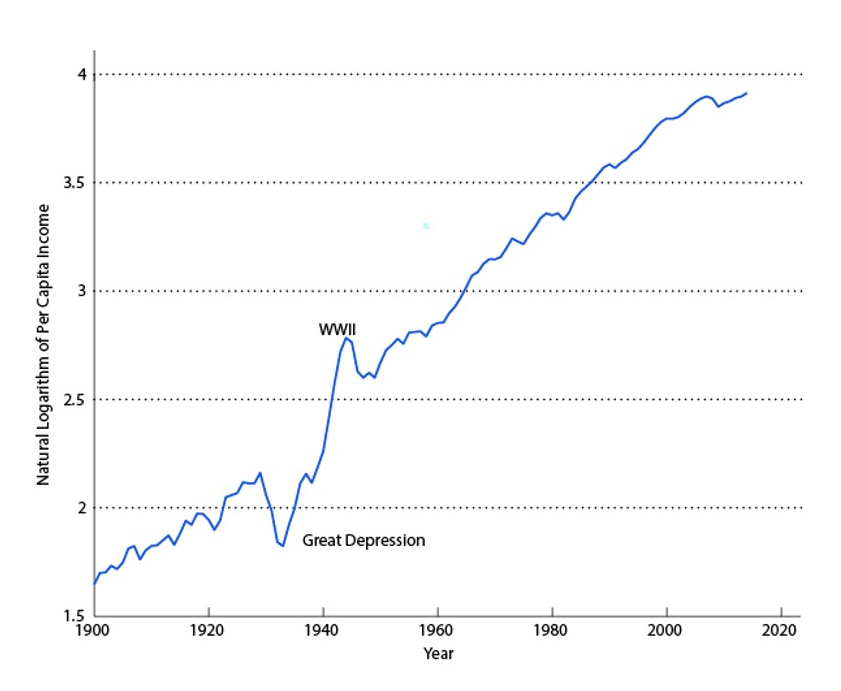
\includegraphics[scale=0.6]{Figures/W_Fig_1pt2.png}
\end{figure}
Takeaways:  pretty linear, plus some vibrations!  Let's try a trend
\end{frame}

\begin{frame}
\frametitle[alignment=center]{Log Real Per Capita GDP over Time + trend}
\begin{figure}
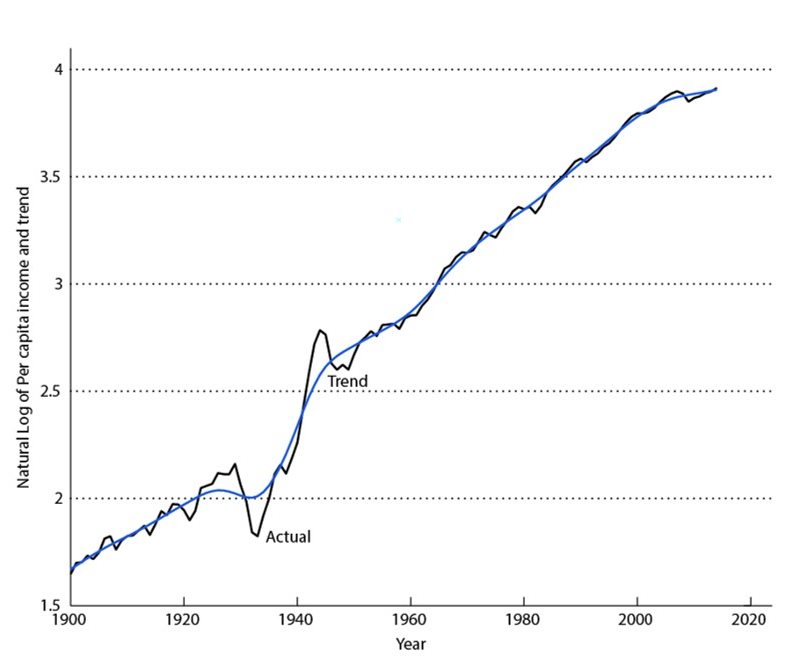
\includegraphics[scale=0.6]{Figures/W_Fig_1pt3.png}
\end{figure}
We can decompose deviation into $$deviation=Data-Trend$$
\end{frame}

\begin{frame}
\frametitle[alignment=center]{Deviations in Log Real Per Capita GDP over Time from Trend}
\begin{figure}
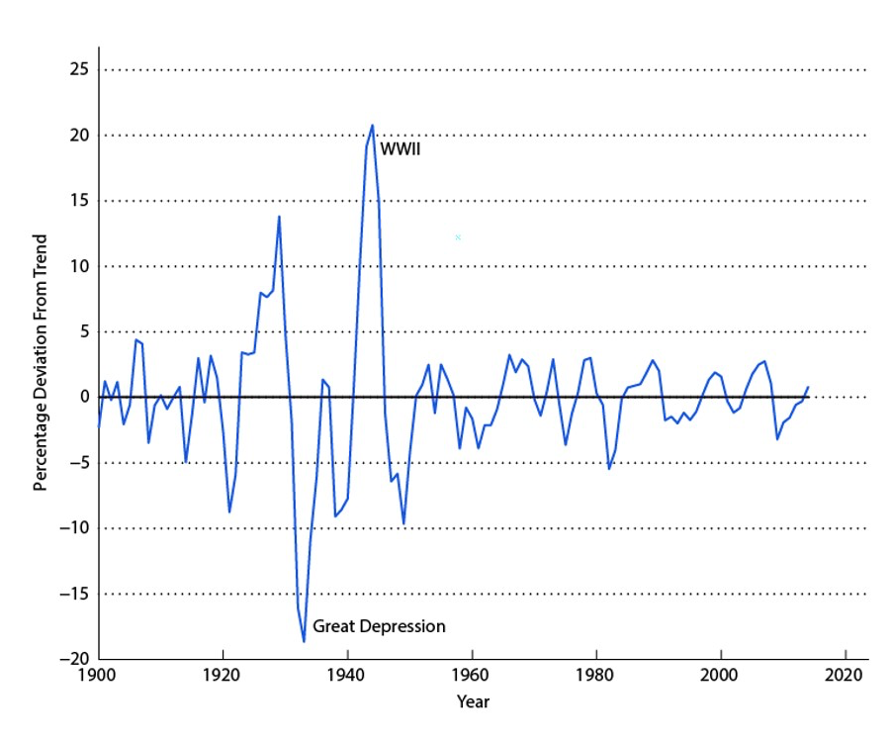
\includegraphics[scale=0.5]{Figures/W_Fig_1pt4.png}
\end{figure}
Post WWII fluctuations fairly muted
\end{frame}

\begin{frame}
\frametitle[alignment=center]{How do we organize our thinking?}
\begin{itemize}
\item We want to do science to it (e.g. testable hypotheses)
\bigskip
\begin{itemize}
\item But not the modern science where you deliberately lie to people and stuff
\end{itemize}
\bigskip
\item But can't run experiments nooooo wat do
\bigskip
\item Astronomy, meteorology have a method:  model it
\bigskip
\item Build up model, find testable implications (both micro and macro)
\bigskip
\item Start from simple idea, build up
\end{itemize}
\end{frame}


\begin{frame}
\frametitle[alignment=center]{Macro Model Building}
\begin{itemize}
\item We need:
\begin{itemize}
\item Consumers \& firms interacting in economy
\item Set of goods consumers wish to consume
\item Consumer's preferences over goods
\item Technology available to firms for producing goods
\item Resources available
\end{itemize}
\item With these pieces, we start putting things togeher.  Assume for instance
\begin{itemize}
\item Consumers and firms optimize:  they don't randomly consume or produce
\item Implies economy is in a ``competitive equilibrium"
\end{itemize}
\item Competitive equilbrium:  goods are bought and sold on markets in which consumers and firms are price takers:  they don't act as though their actions have an affect on market prices (though they may)
\item Once we build the model, we can ask it questions: can it explain the data?
\item Once it can explain the data: can it forecast the data?  What would the world look like if we changed policy?
\end{itemize}
\end{frame}

\begin{frame}
\frametitle[alignment=center]{Microeconomic Principles}
\begin{itemize}
\item Building up from micro principles very important in macro!
\bigskip
\item But why?
\bigskip
\item Akin to building up engineering from molecules:  is that really necessary?
\bigskip
\item Yes!  In this world, when government changes rules, molecules change their behavior
\bigskip
\item Fundamental idea in Macro is the ``Lucas Critique:"  macroeconomic policy analysis can only be done sensibly if microeconomic behavior is taken into account
\end{itemize}
\end{frame}


\begin{frame}
\frametitle[alignment=center]{Disagreement in Macroeconomics}
\begin{itemize}
\item Most of what we learn in macro is not contested (you only hear about the contested parts!)
\bigskip
\item Solow Growth model and endogenous growth models is a way of showing what matters and what doesn't in growth, and aren't very controversial
\bigskip
\item However, business cycle modeling is!  
\begin{itemize}
\item Old Keynesian:  wages and prices are sticky in short run, and government intervention can correct inefficiencies (but non-micro)
\item Modern real business cycle theory:  real fluctuations can be (may be) optimal or responses to real events and government intervention is inefficient or even harmful
\item New Keynesian:  try to integrate the two!
\end{itemize}
\end{itemize}
\end{frame}

\begin{frame}
\frametitle[alignment=center]{Twelve Key Concepts in Williamson}
\begin{enumerate}
\item What is produced and consumed in the economy is determined jointly by the economy's productive capacity and the preferences of consumers
\item In free market economies, there are strong forces that tend to produce socially efficient economic outcomes
\item Unemployment is painful for individuals, but is a necessary evil in modern economies
\item Improvements in a country's standard of living are brought about in the long run by technological progress
\item A tax cut is not a free lunch
\item Credit markets and banks play key roles in the macroeconomy
\end{enumerate}
\end{frame}

\begin{frame}
\frametitle[alignment=center]{Twelve Key Concepts in Williamson}
\begin{enumerate}\addtocounter{enumi}{6}
\item What consumers and firms anticipate for the future has an important bearing on current macroeconomic events
\item Money takes many forms, and society is much better off with it than without it.  Once we have it, however, changing its quantity ultimately does not matter
\item Business cycles are similar, but they can have many causes
\item Countries gain from trading goods and assets with each other, but trade is also a source of shocks to the domestic economy
\item In the long run, inflation is caused by growth in the money supply
\item If there is a short-run trade-off between output and inflation, that has very different implications relative to the relationship between nominal interest rates and inflation
\end{enumerate}
\end{frame}


\begin{frame}
\frametitle[alignment=center]{Current Macroeconomic Events}
\begin{itemize}\addtocounter{enumi}{6}
\item We looked at GDP, let's look at some of the other macroeconomic time series we want to understand!
\end{itemize}
\end{frame}


\begin{frame}
\frametitle[alignment=center]{Productivity}
\begin{figure}
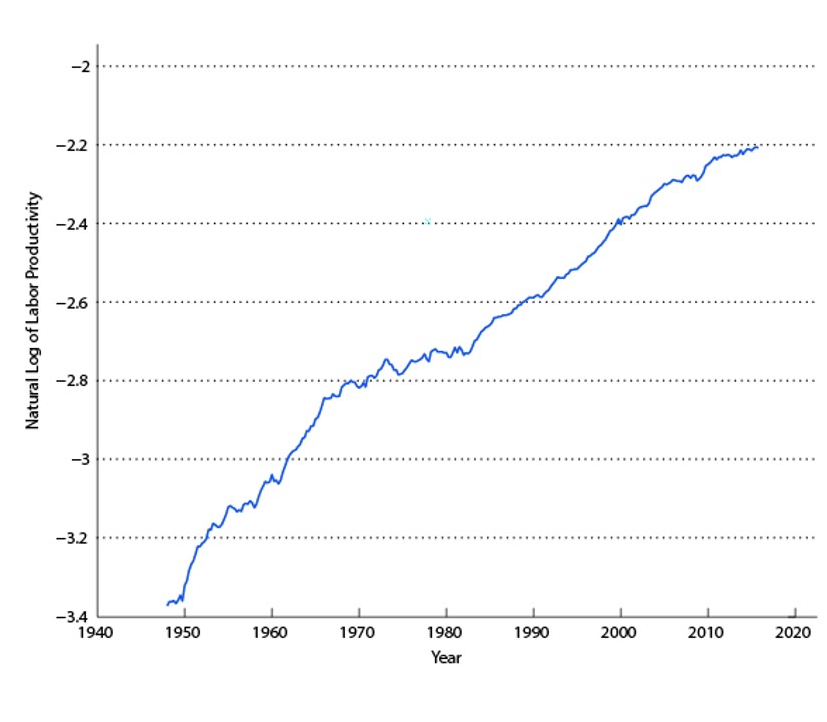
\includegraphics[scale=0.6]{Figures/W_Fig_1pt5.png}
\end{figure}
\end{frame}


\begin{frame}
\frametitle[alignment=center]{Unemployment Rate}
\begin{figure}
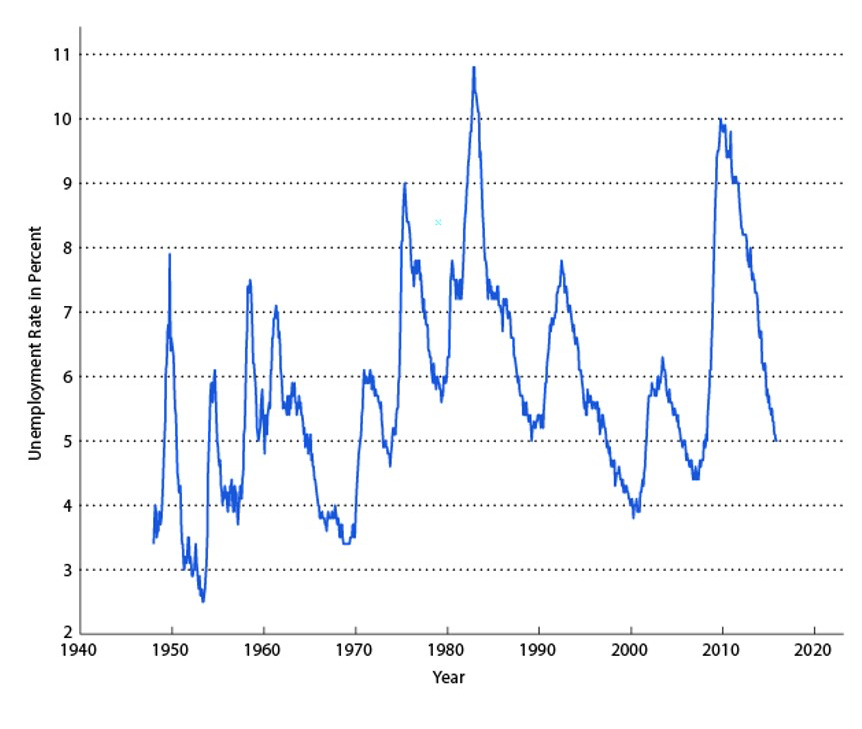
\includegraphics[scale=0.6]{Figures/W_Fig_1pt6.png}
\end{figure}
\end{frame}

\begin{frame}
\frametitle[alignment=center]{Unemployment and Vacancies}
\begin{figure}
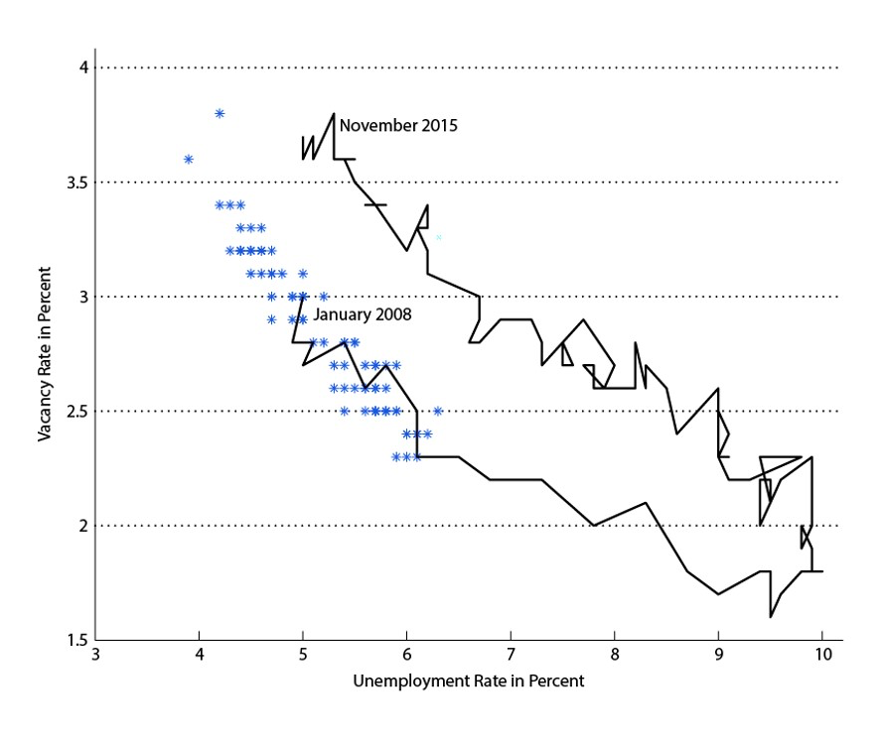
\includegraphics[scale=0.6]{Figures/W_Fig_1pt7.png}
\end{figure}
\end{frame}


\begin{frame}
\frametitle[alignment=center]{Taxes and Spending}
\begin{figure}
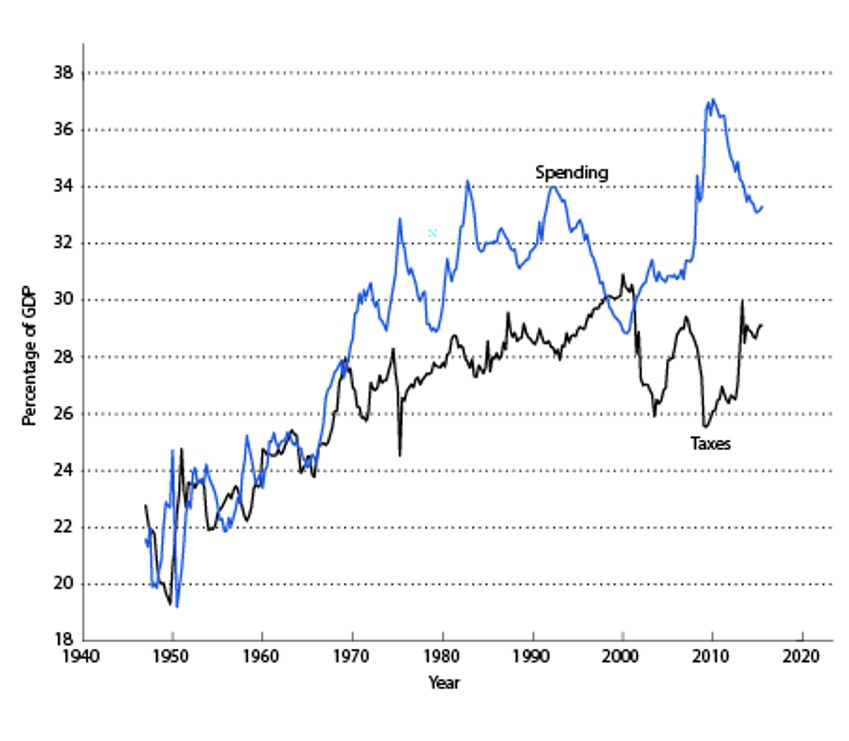
\includegraphics[scale=0.6]{Figures/W_Fig_1pt8.png}
\end{figure}
\end{frame}

\begin{frame}
\frametitle[alignment=center]{Government Surplus}
\begin{figure}
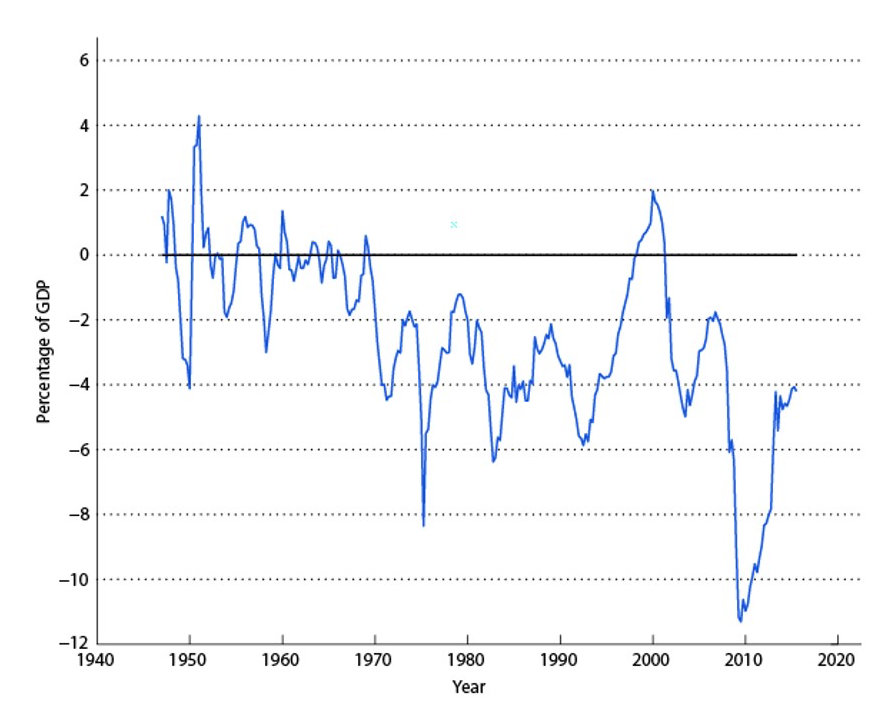
\includegraphics[scale=0.6]{Figures/W_Fig_1pt9.png}
\end{figure}
\end{frame}

\begin{frame}
\frametitle[alignment=center]{Inflation Rate}
\begin{figure}
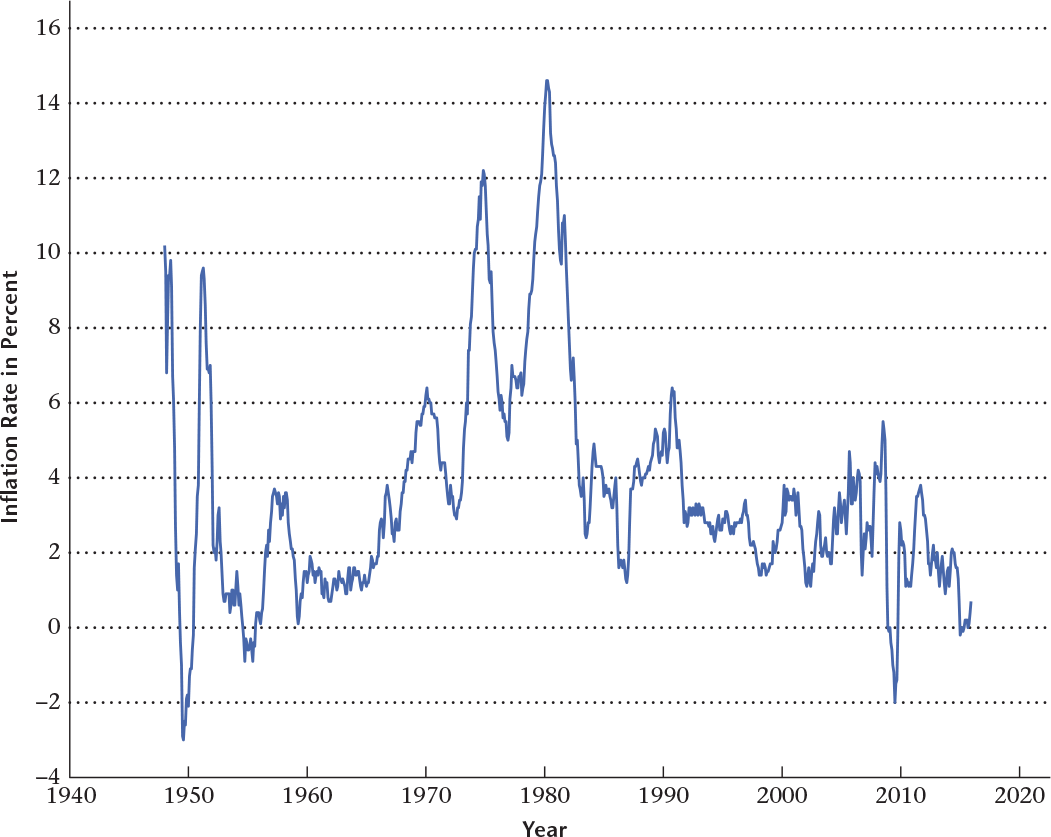
\includegraphics[scale=0.6]{Figures/W_Fig_1pt10.png}
\end{figure}
\end{frame}

\begin{frame}
\frametitle[alignment=center]{Nominal Interest Rate and Inflation Rate}
\begin{figure}
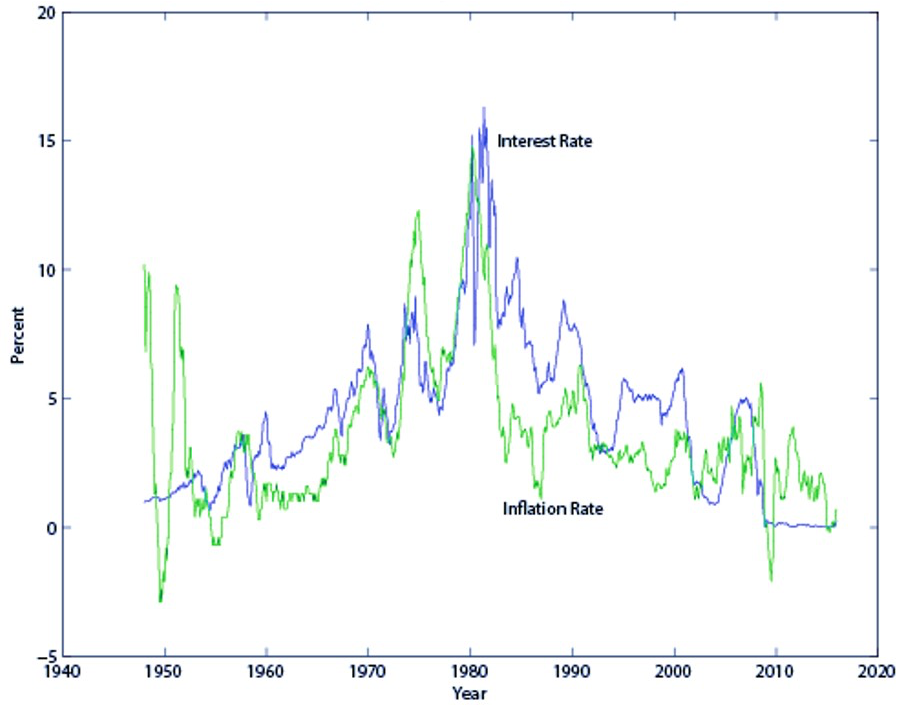
\includegraphics[scale=0.6]{Figures/W_Fig_1pt11.png}
\end{figure}
\end{frame}

\begin{frame}
\frametitle[alignment=center]{Real Interest Rate}
\begin{figure}
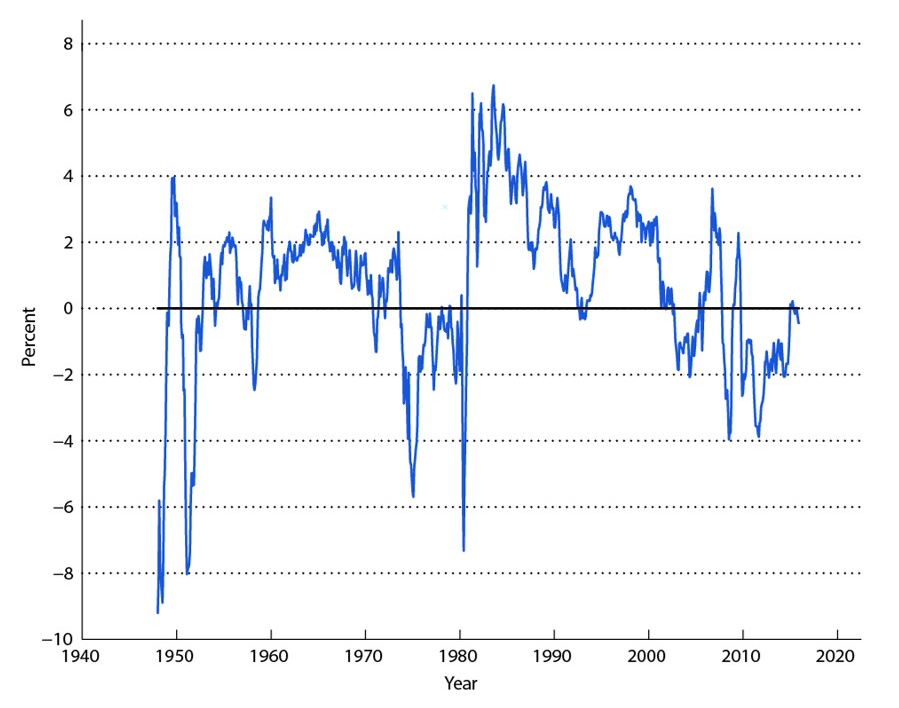
\includegraphics[scale=0.6]{Figures/W_Fig_1pt12.png}
\end{figure}
\end{frame}

\begin{frame}
\frametitle[alignment=center]{Business Cycles in U.S.}
\begin{figure}
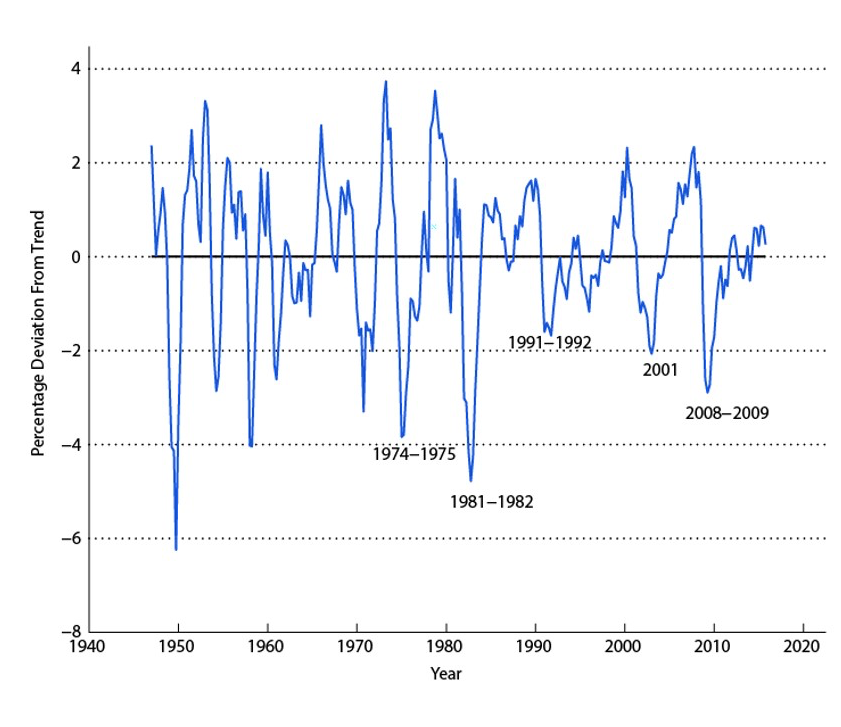
\includegraphics[scale=0.6]{Figures/W_Fig_1pt13.png}
\end{figure}
\end{frame}


\begin{frame}
\frametitle[alignment=center]{Interest Rate Spread}
\begin{figure}
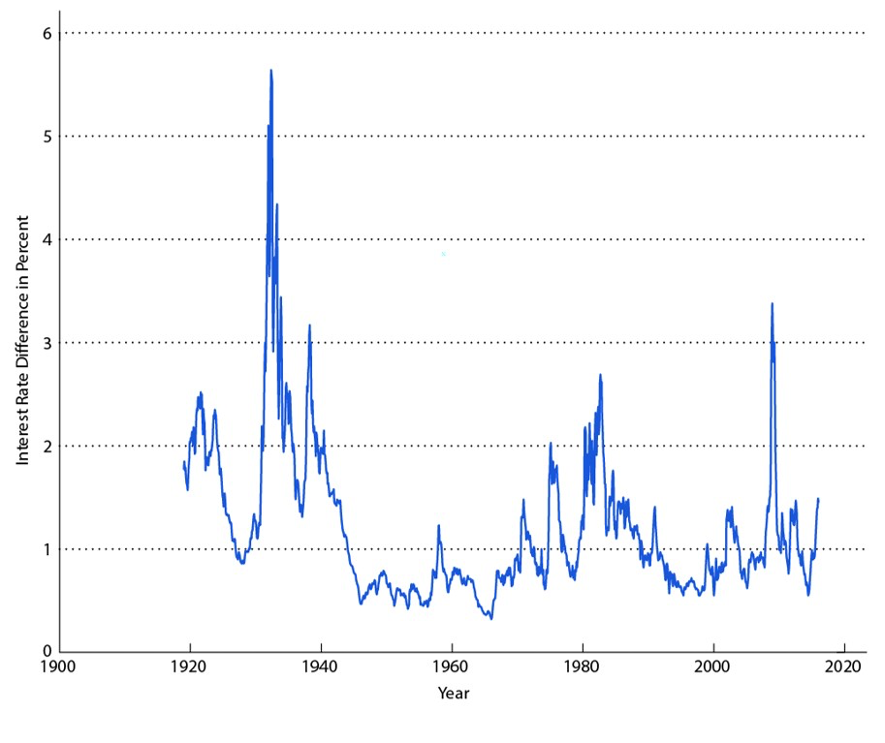
\includegraphics[scale=0.6]{Figures/W_Fig_1pt14.png}
\end{figure}
\end{frame}

\begin{frame}
\frametitle[alignment=center]{Interest Rate Spread}
\begin{figure}
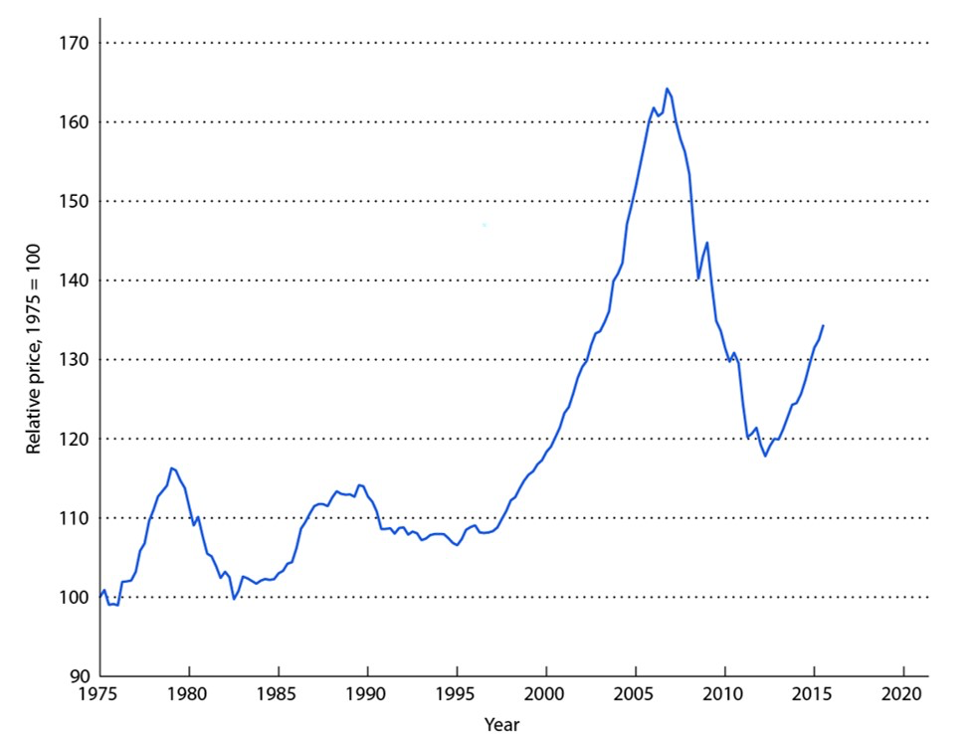
\includegraphics[scale=0.6]{Figures/W_Fig_1pt15.png}
\end{figure}
\end{frame}

\begin{frame}
\frametitle[alignment=center]{Exports and Imports of Goods and Services as Percentages of GDP}
\begin{figure}
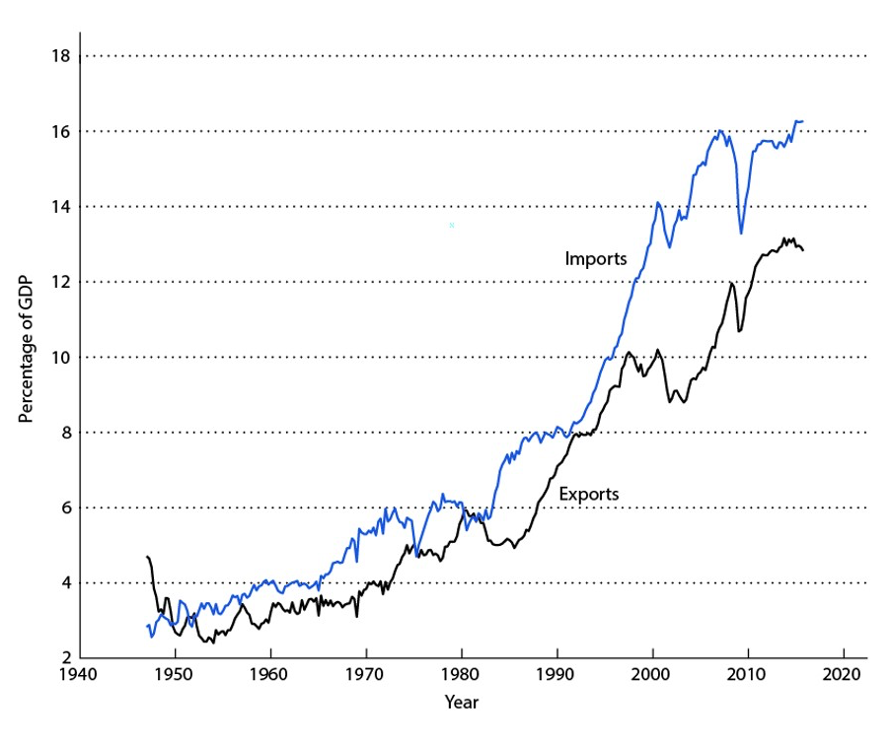
\includegraphics[scale=0.6]{Figures/W_Fig_1pt16.png}
\end{figure}
\end{frame}

\begin{frame}
\frametitle[alignment=center]{Relative Price of Housing}
\begin{figure}
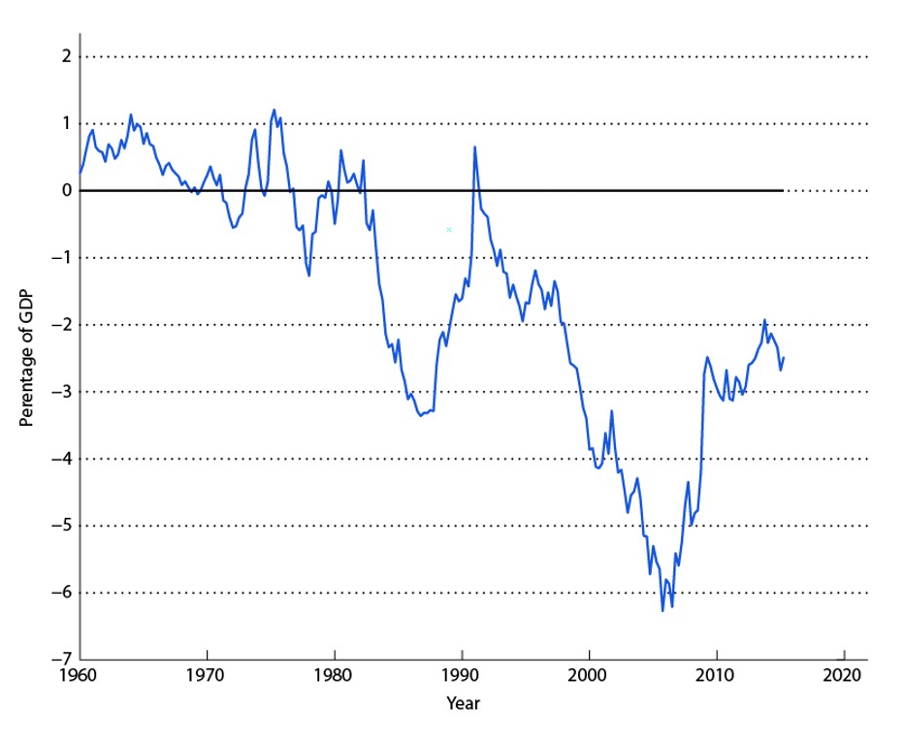
\includegraphics[scale=0.6]{Figures/W_Fig_1pt17.png}
\end{figure}
\end{frame}

\begin{frame}
\frametitle[alignment=center]{Summary}
\begin{itemize}
\item Modern macro builds up models from microeconomic principles
\bigskip
\item We want to build up a model that can explain the phenomena we see
\bigskip
\item With it, we can give policy advice!

\end{itemize}
\end{frame}


\end{document}